\section{The methods on the open models}
\label{app:trained}

DAgger trains Qwen3.5-9B on the stream, each run on a node of eight H100 GPUs rented for it. A vLLM server on the node serves the base model and every adapter by name, and the student plays every move through prime-agent 0.9.6 under the same rules as method Q. It samples at the setting of Qwen3.5-9B's model card for thinking mode (temperature 1, top-$p$ 0.95, top-$k$ 20, presence penalty 1.5), as do the untrained student that DAgger is read against and the student told the page alone (Appendix~\ref{app:told}): at temperature 1 with no truncation, as the methods served through OpenRouter sample, a trained adapter's replies ran into incoherent text up to the token cap, which they never did at the card's setting. Every model call is saved as it was served, and every game's outcome goes to the run's records, as for every other method.

\paragraph{The schedule.}
Training waits until the base model has played 24 games. From then on, after each round, a phase trains a LoRA adapter \citep{hu2022lora} of rank 128 and alpha 128 on the query, key, value, output, gate, up and down projections, starting from the last one, on every game the stream has given so far, with one game in ten held out, and it stops once the held-out measure stops improving. The round after next plays with the new adapter, a lag of one round, so that play never waits for training. Every phase's adapter is kept, so the student of any round can be restored and played again. It trains at a learning rate of $10^{-4}$, with 64 of the student's calls to each optimizer step. Its held-out measure is the likelihood of the teacher's labels on the held-out games, taken before the first step and every five steps after it; the phase keeps the adapter at the best of them, and it ends once six in a row have not improved on it, or at 120 steps.

Most of DAgger's phases kept the adapter they started from, since no later measure improved on the first: 152 of the 177 at one user, and 90 of the 100 from round 100. The held-out measure is doing its work there: once the adapter has learned what the games so far teach, further steps only fit the labels it has already seen, and from round 50 at one user the held-out games' negative log-likelihood per token averaged 0.14 to 0.20 above that of the labels the adapter trained on, against 0.02 before. How often a phase still found something to learn grew with the number of users (Figure~\ref{fig:weight-updates}): 25 of the 177 phases changed the adapter at one user, 39 of the 189 at two and about a third at four, where nearly one in three still did after round 100. A single user's stream soon brings little that it has not already taught, so most of its later phases spend their compute and change nothing, while more users bring more new games each round for the student to learn from. The variety of the stream and its size grow together with the users, so the figure does not tell the two apart.

\begin{figure}[htbp]
\centering
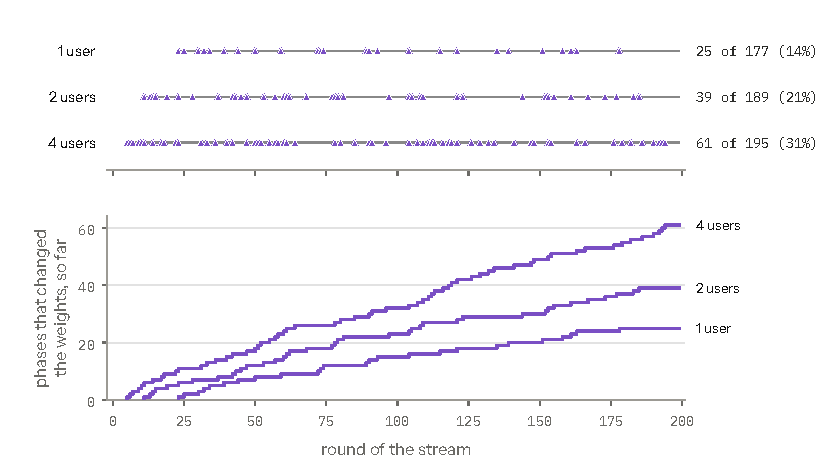
\includegraphics[width=\linewidth]{figures/weight-updates.pdf}
\caption{How often DAgger's phases changed Qwen3.5-9B's adapter at one, two and four users. Above, a triangle marks each round after which the phase kept a later checkpoint than the adapter it started from, on a rule over the rounds that had a phase, which begin once the base model has played 24 games; on the right, how many of the phases did. Below, how many had by each round.}
\label{fig:weight-updates}
\end{figure}

\paragraph{Training and validation loss.}
Figure~\ref{fig:weight-losses} compares the same adapter at the start of each phase: its first training minibatch's loss, before any update, and its validation loss. Validation draws whole games from the accumulated pool to reach about 1,000 labeled calls, with a new sample each phase. The training curve is a minibatch reading, since full training-set evaluations were not logged. Both the data and the student states differ across user counts, so these curves do not establish which learns more on a common test.

\begin{figure}[htbp]
\centering
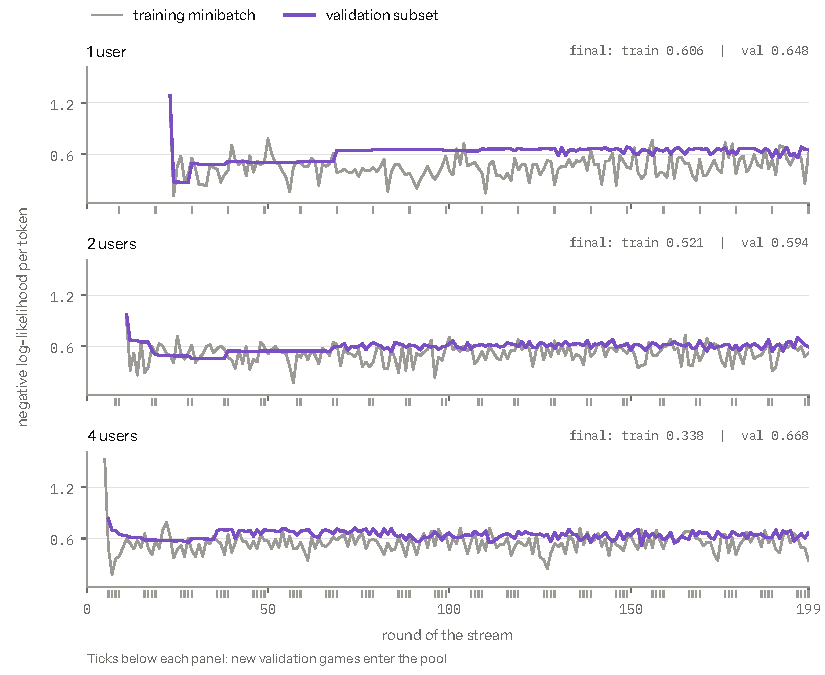
\includegraphics[width=\linewidth]{figures/weight-losses.pdf}
\caption{QDE's training and validation token loss at the start of each phase, with common axes and no smoothing. Ticks mark new games entering the validation pool; its sampled subset can also change between ticks. Values above each panel are from the final phase, which kept its incoming adapter in all three runs.}
\label{fig:weight-losses}
\end{figure}

\paragraph{DAgger with an expert-guided teacher (DE).}
In each state that the student met, the teacher, GLM-5.3 Flash at medium effort, is asked for its own reply, reading the playing rules alone, the expert guidance without its program-library procedure. Its reply, reasoning included, is the target of a supervised loss on the student's own context \citep{ross2011dagger}. Methods QE and GE receive those rules plus the program-library procedure (Appendix~\ref{app:prompts}). DAgger's student sees neither directly. At one user the teacher was asked about 21,096 of the student's moments, and 21,047 of its replies became training examples: 39 moments got no label after every re-ask, and 10 labels did not render. It took 1.07 asks per label, and 94\% of labels came at the first ask.

\paragraph{Other weight-based methods.}
\label{app:other-weights}
We also trained the student by a policy gradient on each game's outcome \citep{schulman2017ppo} and by self-distillation from the teacher's move \citep{shenfeld2026sdft}, but got neither learning reliably. The policy gradient, learning only from the games the student wins, stalled after its few early wins; in self-distillation the student often read the teacher's move inside the tool's output as a move already made, learned that and played worse than untrained.

\paragraph{How the configuration was chosen.} The search that set DAgger's final configuration scored its candidates on 100 ARC-AGI-1 evaluation tasks that the stream never serves, 23 of which are among the held-out test's, and played some of them on both tests as well. Leaving those 23 tasks out, DAgger saves 0.27 [0.20, 0.34] of the reset's spend on the held-out test at one user and 0.39 [0.32, 0.46] at two, against 0.29 and 0.40 on all 100.

\paragraph{Training compute.}
At one user DAgger ran 177 training phases, one after each round from round 23, for 84.7 hours on two to four of its node's eight H100 GPUs: 263 GPU-hours, \$1,182 at the node's on-demand price of \$4.50 per GPU-hour, and the teacher's labels cost \$71 more. Both are apart from the cost of serving the student, which four other GPUs of the node do.

\paragraph{The page alone.}
\label{app:told}
The untrained student also plays both tests told only the playing rules its teacher reads, wiped before every instance as Q\textsubscript{0} is, four plays of each at the model card's setting, as DAgger and the reset play them. On the held-out test it solves 22 to 33 of the 100 tasks per play, against 13 to 26 untrained and 47 to 52 for DAgger. It answers before seeing a demonstration on 5\% of instances, against 35\% untrained, and DAgger never does; it asks for 1.6 demonstrations per instance and makes 2.2 wrong answers, against 1.1 and 2.5 untrained. It saves 0.09 [0.05, 0.14] of the untrained student's spend, and DAgger 0.19 [0.13, 0.26] more. On the seen test, where it keeps nothing of the stream, it saves 0.16 [0.08, 0.26], against DAgger's 0.57 [0.48, 0.67], DAgger 0.41 [0.32, 0.50] more.

\paragraph{The teacher on solved instances.}
Table~\ref{tab:solved} gives GLM-5.3 Flash's methods from round 100, when every task has been met, as Section~\ref{sec:results} reads them, beside its stateless floor.

\begin{table}[htbp]
\centering
\footnotesize\setlength{\tabcolsep}{3pt}
\begin{adjustbox}{max width=\linewidth}
\begin{tabular}{lrr@{\hspace{0.4em}}lrrr}
\toprule
system & solved (\%) & \multicolumn{2}{c}{budget a solve used (\%)} & solved at no cost (\%) & demonstrations & wrong answers \\
\midrule
\multicolumn{7}{l}{\emph{GLM-5.3 Flash (medium), prime-agent}} \\
GC\textsubscript{0} & 83 & 20.5 & {\scriptsize [16.0, 25.7]} & 0 & 1.8 & 1.5 \\
G\textsubscript{0} & 93 & 17.5 & {\scriptsize [14.3, 20.7]} & 0 & 1.9 & 0.9 \\
G & 94 & 13.6 & {\scriptsize [9.3, 18.3]} & 23 & 1.4 & 0.7 \\
GA & 98 & 16.0 & {\scriptsize [12.4, 20.0]} & 9 & 1.7 & 0.9 \\
GE & \textbf{99} & 4.6 & {\scriptsize [2.8, 6.3]} & 74 & 0.4 & 0.3 \\
GP & \textbf{99} & \textbf{1.4} & {\scriptsize [0.3, 2.9]} & \textbf{92} & \textbf{0.1} & \textbf{0.1} \\
\bottomrule
\end{tabular}

\end{adjustbox}
\caption{GLM-5.3 Flash in prime-agent, rounds 100 to 199 of the stream at one user: the share of instances solved, the budget a solve used in percent of the budget with its 95\% interval over task resamples, the share of solves that used none of it, and the demonstrations and wrong answers behind a solve. Perfect memory on any of these systems spends nothing here. Bold marks each column's best.}
\label{tab:solved}
\end{table}

\paragraph{The two tests in absolute terms.}
A share saved is a share of the reset's own spend, so a learner whose reset already spends little can save a large share of very little, and a share is read beside the budgets it comes from. Table~\ref{tab:tests-absolute} gives every method of Table~\ref{tab:tests} in those terms: the budget used on each test and the share of the held-out test solved, the learner's own beside the reset's.

\begin{table}[htbp]
\centering
\footnotesize\setlength{\tabcolsep}{4pt}
\begin{adjustbox}{max width=\linewidth}
\input{\hoped{sections/tables/tests-absolute}}
\end{adjustbox}
\caption{Every method at one user in absolute terms, on Qwen3.5-9B (left) and on GLM-5.3 Flash (right): $U$ is the budget used on a test in percent, lower is better, and $P_{\mathrm{held}}$ the share of the held-out test solved in percent, each the mean of \testPlays{} plays, the learner's own in normal type and the reset's beside it in small type, each marked with an asterisk where it is above the bare model's, the stateless floor's, as Appendix~\ref{app:heldout} flags. Table~\ref{tab:tests} gives each method's share saved, which is one minus the ratio of the two budgets. Bold marks each column's best.}
\label{tab:tests-absolute}
\end{table}

\paragraph{DAgger at every number of users.}
Table~\ref{tab:tests-users} gives DAgger on Qwen3.5-9B with its floors and wiped learners at each number of users it served, as Table~\ref{tab:tests} gives the methods at one user. At two and four users every user brings 25 tasks of their own, and each method plays the stream and each test once, as does its wiped twin at the same number of users, which it is read against, except that DAgger plays each test \testPlays{} times and its twin the seen test \testPlays{} times. The seen test then serves every user's own tasks, so only that twin played its instances. The held-out test is the same at any number of users, so there the twin's one play joins the \testPlays{} plays of the method's reset at one user, the same wiped system. A method that keeps nothing is its own reset, with no second play of the seen test to be read against at two or four users, and the table gives it at one user alone.

\begin{table}[htbp]
\centering
\footnotesize\setlength{\tabcolsep}{3pt}
\input{\hoped{sections/tables/tests-users}}
\caption{DAgger on Qwen3.5-9B, and its baselines, at each number of users they served, read as in Table~\ref{tab:tests}: the share learned on the stream and the share saved on each frozen test, against the method's wiped twin at the same number of users, and on the held-out test against the reset's plays at one user as well. At two and four users DAgger plays each test \testPlays{} times, and its baselines once. Bold marks each column's best among the values whose 95\% interval lies above zero.}
\label{tab:tests-users}
\end{table}

\paragraph{Why four users saved no more than two.}
On the held-out test DAgger saved 0.40 [0.34, 0.47] at two users and 0.39 [0.33, 0.46] at four (Table~\ref{tab:tests-users}), although four users gave it the games of twice as many tasks. We think the brake was the stream's training procedure, not the games. A phase measures its adapter every five steps and stops after six measures without a gain, so a phase that finds no gain within 30 steps stops at any number of users, while the games it trains on grow with the users: 30 steps are about a tenth of a pass over one user's final labels, but a fiftieth over four users'. Rolling back to each phase's best, the runs kept 760 of their 6,060 steps at one user, 1,375 of 7,010 at two and 2,147 of 7,852 at four, about 2.5, 1.9 and 1.4 passes over their final 19,243, 46,744 and 97,580 labels. To test this, we trained the student once more from the base model on all of each run's final labels, shuffled, with no phases, warm starts or rollbacks, at the run's learning rate, batch and held-out games. It measured about eight times a pass and stopped after eight measures without a gain, and its best adapter, reached after about two passes at every number of users, played both tests from the run's own end-of-stream memory, four times at four users and once at one and two. At one and two users the fit saved what its run did on the held-out test (the fit less the run, $-0.01$ [$-0.08$, 0.06] and $-0.01$ [$-0.09$, 0.07]). At four users, where the run had kept the fewest passes, the fit saved $S_{\mathrm{held}} = 0.46$ [0.40, 0.53], 0.07 [0.02, 0.13] more than its run and 0.06 [0.01, 0.11] more than two users' run, and $S_{\mathrm{seen}} = 0.59$ [0.53, 0.66], 0.08 [0.04, 0.12] more than its run. The held-out loss did not show this: each fit's best was about 3\% below its run's last at every number of users. So four users' games held more than the stream's procedure drew from them. Whether they hold more than two users' games fit the same way is not yet measurable, at 0.07 [$-0.01$, 0.15] from the two-user fit's one play, and whether generalization keeps growing with more users, up to all 400 of ARC-AGI-1's training tasks at 16 users, we leave to future work.

\paragraph{Forgetting.}
\label{app:forgetting}
Every task of the stream is visited eight times at any number of users, in a burst whose rounds differ from task to task: at one user the first task's visits end at round 44 and the second's at round 160. A task's last visit therefore says how long it went unpracticed before the seen test, with practice held equal. We read each task's share saved on the seen test against the reset on the same task, so that the task's difficulty cancels, and compare the tasks visited most recently with those left longest (Figure~\ref{fig:forgetting}). No method forgot measurably. DAgger shows no measurable gap at one, two or four users. At four users, with 100 tasks, the half of the tasks visited last saved 0.55 and the half left longest 0.47, a gap of 0.08 [$-0.05$, 0.21], as replaying every game in each phase should give. Over the ten methods whose $S_{\mathrm{seen}}$ is above zero, splitting the tasks into halves and quarters by their last and by their first visit, and taking the slope on each, 4 of 70 readings exclude zero, about what chance alone gives. The largest, GC's, cannot be forgetting, since the demo cache keeps each task's pairs and never drops one: it comes from two tasks of its oldest quarter that a cache of pairs barely helps with, on which QC saved as little (\texttt{scripts/forgetting.py}).

\begin{figure}[htbp]
\centering
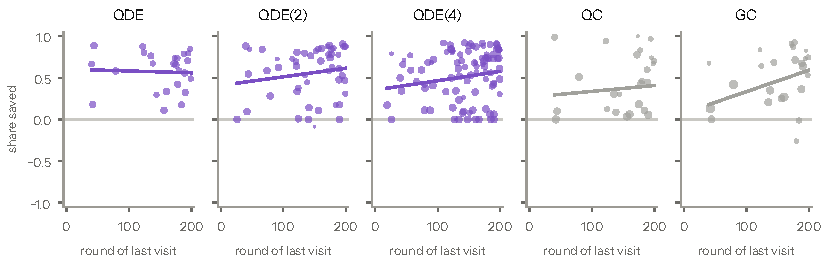
\includegraphics[width=\linewidth]{figures/forgetting.pdf}
\caption{Each task's share saved on the seen test against the round of its last visit in the stream, for DAgger at one, two and four users and for the two demo-cache floors. A dot's area is the reset's spend on the task, and each line is the fit weighted by it.}
\label{fig:forgetting}
\end{figure}
